\documentclass{minimal}
\usepackage{tikz}
\usetikzlibrary{calc}
\begin{document}
    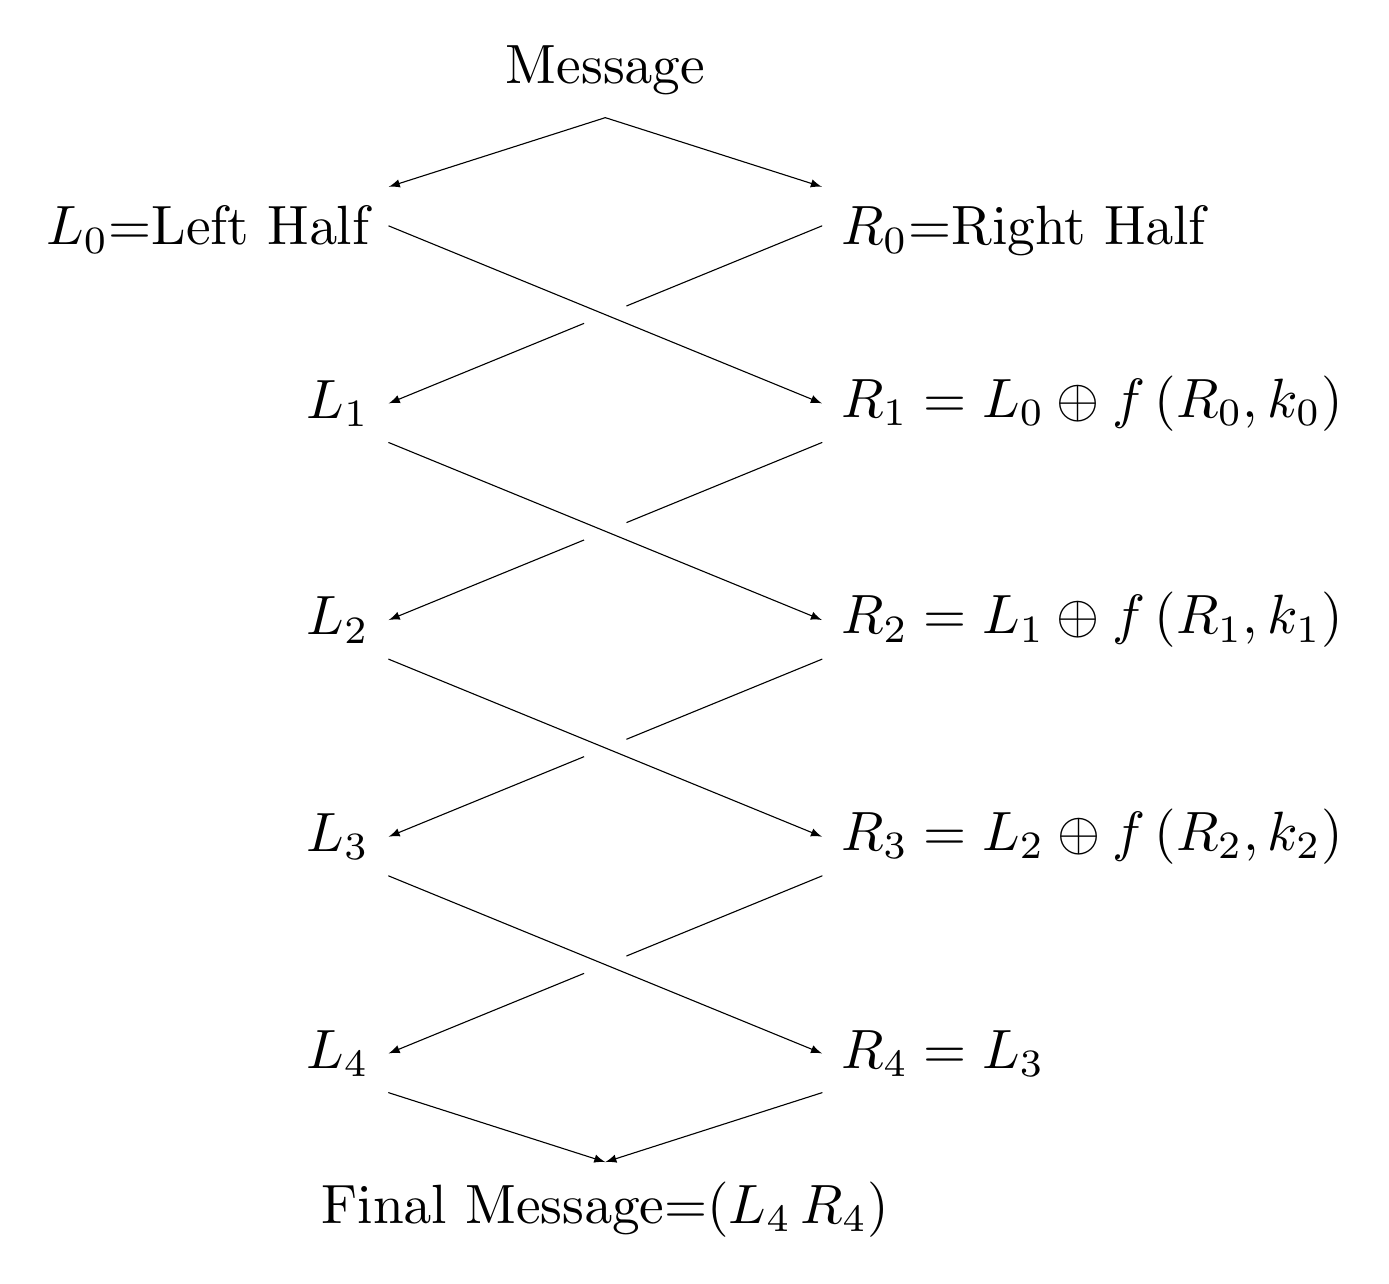
\begin{tikzpicture}[scale=2.75,cap=round,>=latex,every node/.style={scale=2}]
        \node (start) at (0,0){};
        \node (left) at (-1,-0.5){};
        \node (right) at (1,-0.5){};
        \draw (start.center) node[yshift=5pt]{Message};
        \draw[->] (start.south) -- (left.north) node[anchor=north east]{$L_0$=Left Half};
        \draw[->] (start.south) -- (right.north) node[anchor=north west]{$R_0$=Right Half};
        \foreach \dy in {1,...,3}{
            \node (templ) at ($(left)+(0,-1)$){};
            \node (tempr) at ($(right)+(0,-1)$){};
            \pgfmathparse{int(\dy-1)}\let\pr=\pgfmathresult;
            \draw[->] (right.south) -- (templ.north) node[anchor=east]{$L_\dy$};
            \fill[color=white] ($(right)!0.5!(templ)$) circle (3pt);
            \draw[->] (left.south) -- (tempr.north) node[anchor=west]{
                $R_\dy=L_\pr\oplus f\left(R_\pr,k_\pr\right)$
            };
            \node (right) at (tempr){};
            \node (left) at (templ){};
        }
        \node (templ) at ($(left)+(0,-1)$){};
        \node (tempr) at ($(right)+(0,-1)$){};
        \draw[->] (right.south) -- (templ.north) node[anchor=east]{$L_4$};
            \fill[color=white] ($(right)!0.5!(templ)$) circle (3pt);
        \draw[->] (left.south) -- (tempr.north) node[anchor=west]{$R_4=L_3$};
        \node (right) at (tempr){};
        \node (left) at (templ){};
        \node (templ) at ($(left)+(0,-0.5)$){};
        \node (tempr) at ($(right)+(0,-0.5)$){};
        \node (finish) at ($(templ)!0.5!(tempr)$){};
        \draw[->] (right.south) -- (finish.north);
        \draw[->] (left.south) -- (finish.north);
        \node[yshift=-5pt] at (finish) {Final Message=$(L_4\, R_4)$};
    \end{tikzpicture}

\end{document}